\section{Better Exploiting Linguistic Features}
\label{ch:improvements:our_app}
As discussed by \newcite{moosavi17b},
there is a large lexical overlap between the coreferring mentions
of the CoNLL training and evaluation sets.
As a result, lexical features provide a very strong signal for resolving coreference relations.

For linguistic features to be more effective in current coreference resolvers,
which rely heavily on lexical features,
they should also provide a strong signal for coreference resolution.
% such that they would not be undermined in the presence of lexical features.

Additional linguistic features are not necessarily all informative for coreference resolution, especially if they are extracted automatically and are noisy.
Besides, for features with multiple values, e.g.\ mention-based features, 
only a small subset of values may be informative.

To better exploit linguistic features, 
we only employ (feature, value) pairs\footnote{Henceforth, we refer to them as feature-values.} 
that are informative for coreference resolution.
Coreference resolution is a complex task in which features have complex interactions \cite{recasens09}.
As a result, we cannot determine the informativeness of feature-values in isolation.

We use a discriminative pattern mining approach \cite{cheng07,cheng08,batal10}
that examines all combinations of feature-values, up to a certain length, 
and determines which feature-values are informative when they are considered in combination.
%\footnote{the similarity and differences of using discriminative pattern mining vs. standard feature selection algorithms is explained in the supplementary materials}

Due to the large data size (all mention-pairs of the CoNLL training data)
and the high dimensionality of 
feature-values, compared to common evaluation sets of pattern mining methods, 
the existing discriminative pattern mining approaches were not applicable to our data.
In this section, we propose an efficient discriminative pattern mining approach, called Efficient Pattern Miner (EPM), that is scalable to large NLP datasets. 
The most important properties of EPM are (1) it examines all frequent feature-values combinations, up to the desired length, 
(2) it is scalable to large datasets, and (3) it is only data dependent and independent of the coreference resolver.
%
%\subsection{Determining Informative Feature-Values}
%\label{ch:improvement:pattern}
%and \newcite{li01}).
%Mining a discriminative and non-redundant set of patterns from labeled data is referred to as supervised pattern set mining.
%There are various studies showing that the incorporation of these patterns 
%as features significantly improves the performance \cite{cheng07,cheng08,batal10}.
%Assume the data is represented by a set of features. 
%Let a pattern be the set of one or more feature-values.
%In this way, a pattern is a form of non-linear feature combination over individual features.
%Patterns can be more informative and are likely to capture the underlying semantics better than individual features \cite{cheng07}.
%TODO Supervised pattern set mining approaches, e.g.\ \newcite{bring09}, \newcite{novak09}, \newcite{zimmer14}, inter alia, 
%are mainly grouped in two categories: 
%(1) post-processing, and (2) iterative approaches.
%TODO Post-processing approaches first mine a set of patterns satisfying certain constraints,
%which is usually the minimum frequency. 
%The mining step is then followed by a post-processing step which selects a subset of mined patterns based on discriminative power and redundancy criteria.
%Iterative approaches mine one or more patterns satisfying certain constraints.
%Based on the selected pattern(s) they modify the constraints or data and then repeat the mining process.
%TODO In natural language processing tasks, 
%it is often the case that the dataset is very large and the data includes a large set of feature-values.
%Therefore, efficiency is a main concern for applying a pattern mining approach to NLP tasks.
%TODO Post-processing approaches are generally faster 
%than iterative ones because they only need one iteration of the mining process.
%TODO However, the post-processing approaches are still not efficient enough for large data sizes or large search spaces.
%Enumerating all frequent patterns of data has been proven to be an NP-complete problem \cite{yang06}.
%Besides, when the search space is large, 
%the mining step may result in a huge number of patterns,
%which in turn makes post-processing also a time-consuming step.
%We consider two variations of the discriminative power and redundancy measures: 
%(1) lenient variants that are directly checked during the mining step on individual patterns,
%and (2) strict variants that are checked in the post-processing step.
%Since we also use lenient variations of discriminative power and redundancy measures during the mining step,
%the number of patterns for the post-processing step decreases considerably and therefore the time efficiency of the whole algorithm increases
%
\subsection{Notation}
\label{sect:back}
We use the following notations and definitions throughout this section:
\squishlist
\item $D=\{X_i,c(X_i)\}_{i=1}^n$: set of $n$ training samples. 
$X_i$ is the set of feature-values that describes the $i$th sample. 
$c(X_i) \in C$ is the label of $X_i$, e.g.\ coreferent and non-coreferent.
\item $A=\{a_1,\dots,a_l\}$: set of all feature-values present in $D$.
Each $a_i \in A$ is called an item, e.g.\ $a_i=$``anaphor type=proper''.
\item $p$: pattern $p=\{a_{i_1},\dots, a_{i_k}\}$ is a set of one or more items, e.g.\ $p=$\{``anaphor type=proper'', ``antecedent type=proper''\}. 
%e.g.\ \{``anaphor type=proper'', ``head match=true''\}.
%In other words, pattern is a compositional feature that combines primitive features.
%\item $D_p=\{X_i|p\in X_i\}$: the set of samples that is matched by pattern $p$. 
%referred to as cover $p$.
\item $support(p,c_i)$: the number of samples that contain pattern $p$ and are labeled with $c_i$. 
%i.e. $|\{X_i | X_i \in D_p \land c(X_i)=c_i\}|$.
%\item $\hat c(p)$:
%we are interested in patterns that are predictive of output labels ($C$).
%$Pr(c_i|p)$ 
%is equal to the posterior probability of $c_i$ in $D_p$. 
%We consider the estimated class of pattern $p$ as 
%$\hat c(p) = \arg\max_{c_i \in C}Pr(c_i|p)$. 
%\item Super-pattern:
%pattern $q$ is a super-pattern of $p$ if $\forall a_i \in p : a_i \in q$. 
\squishend

\subsection{Data Structure}
\label{fptree}
For representing the input samples, we use the Frequent Pattern Tree (FP-Tree) structure that is the data structure of the FP-Growth algorithm \cite{han04}, i.e.\ one of the most common algorithms for frequent pattern mining.
FP-Tree provides a structure for representing all existing patterns of data in a compressed form.
Using the FP-Tree structure allows an efficient enumeration of all frequent patterns.
In the FP-Tree structure, items are arranged in descending order of frequency.
Frequency of an item corresponds to $\sum_{c_i \in C} \: support(a_i, c_i)$.
%, i.e.\ the frequency of the item $a_i$ in all class labels.
Except for the root,
which is a null node,
each node $n$ contains an item $a_i \in A$.
It also contains the support values of $a_i$
in the subpath of the tree that starts from the root and ends with $n$, i.e.\ $support_n(a_i,c_j)$.  

The FP-Tree construction method \cite{han04} is as follows:
(a) scan $D$ to collect the set of all items, i.e.\ $A$. 
 Compute $support(a_i,c_j)$ for each item $a_i \in A$ and label $c_j \in C$.
Sort $A$'s members in descending order according to their frequencies, i.e. $\sum_{c_i \in C} \: support(a_i, c_i)$. 
(b) create a null-labeled node as the root, and (c) scan $D$ again. For each $(X_i, c(X_i)) \in D$: 
\begin{enumerate}
 \item Order all items $a_j \in X_i$ according to the order in $A$.
 \item Set the current node ($T$) to the root. 
\item \label{prevstep} Consider $X_{i}=[a_k|\bar {X_i}]$, where $a_k$ is the first (ordered) item of $x_{_i}$, 
and $\bar {X_i}=X_i-a_k$.
If $T$ has a child $n$ that contains $a_k$ 
then increment $support_n(a_k,c(X_i))$ by one.
Otherwise, create a new node $n$ that contains $a_k$ with $support_n(a_k,c(X_i))=1$. 
Add $n$ to the tree as a child of $T$. 
\item If $\bar {X_i}$ is non-empty, set $T$ to $n$. 
 Assign $X_i = \bar {X_i}$ and go to step~\ref{prevstep}.  
\end{enumerate}

As an example, assume $D$ contains the following two samples:
\begin{itemize}
 \item [] $X_1$=\{ana-type=NAM, ant-type=NAM, head-match=F\}, $C(X_1)=0$
 \item[]  $X_2$=\{ana-type=NAM, ant-type=NAM, head-match=T\}, $C(X_2)=1$
 %\item[]  $X_4$=\{ana-type=nominal, ana-number=singular, ante-type=nominal, ante-number=singular}\}, $C(X_4)=1$
\end{itemize}
Based on these samples $A$=\{ana-type=NAM, ant-type=NAM, head-match=F, head-match=T\}, $support(a_i,0)_{a_i \in A}$= \{1,1,1,0\}, and $support(a_i,1)_{a_i \in A}$=\{1,1,0,1\}.
If we sort $A$ based on $a_i$'s frequencies ($support(a_i,0)+support(a_i,1)$), the ordering of $A$'s items will remain the same.

The FP-Tree construction steps for the above samples are demonstrated in Figure~\ref{fp-tree_example}.
ana-type, ant-type, and head-match features are abbreviated as
ana, ant, and head, respectively.

\begin{figure}[!htb]
\minipage{0.35\columnwidth}
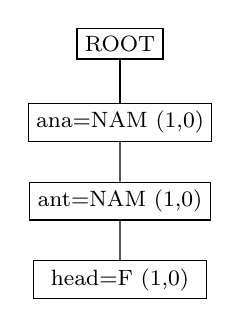
\begin{tikzpicture}
	\footnotesize
\node [rectangle,draw]{ROOT} [level distance=10mm,sibling distance=30mm]
child { node [rectangle,draw]{ana=NAM (1,0)} [level distance=10mm ,sibling distance=15mm]
child {node [rectangle,draw] {ant=NAM (1,0)}
child {node [rectangle,draw,minimum width=22mm] {head=F (1,0)}
}}};
\end{tikzpicture}
\endminipage\hfill
\minipage{0.65\columnwidth}
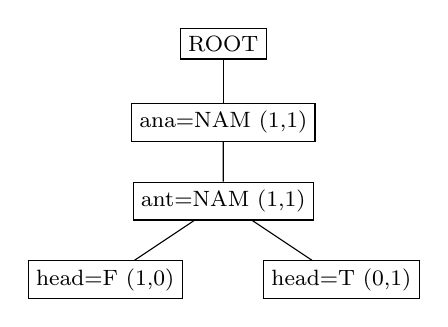
\begin{tikzpicture}
	\footnotesize
	
\node [rectangle,draw]{ROOT} [level distance=10mm,sibling distance=30mm]
child { node [rectangle,draw]{ana=NAM (1,1)} [level distance=10mm ,sibling distance=30mm]
child {node [rectangle,draw] {ant=NAM (1,1)}
child {node [rectangle,draw] {head=F (1,0)}}
child {node [rectangle,draw,minimum width=5mm] {head=T (0,1)}}
}};
\end{tikzpicture}
\endminipage
\caption[FP-Tree construction steps]{Left to right: (partially) constructed FP-Tree for the example in Section~\ref{fptree}.\label{fp-tree_example}}
\end{figure}

%FP-Tree has a header structure that associates each item $a_i$ with a list of pointers to 
%all nodes of the tree that contain $a_i$.
%From this header structure, one can easily obtain $support(a_i,c_j)$ in the whole tree.

%One of the principles used in FP-Growth 
%(i.e. the original algorithm for mining frequent patterns from FP-Tree) \cite{han2000,han04}  
%is that if $p_i$ and $p_j$ are two different patterns, 
%the support values of pattern $p_i \cup p_j$ in the dataset is equal to that of $p_i$ in $D_{p_j}$.
%For instance, Figure~\ref{fp-tree_example} shows a simple FP-Tree that is built based on $D$=\{\{anaphor-type=proper, head-match=T\}, \{anaphor-type=proper, head-match=F\}\}.
%An example of FP-Tree construction method is included in the supplementary materials.

From an initial FP-Tree ($T$) that represents all existing patterns, 
one can easily obtain a new FP-Tree in which all patterns include a given pattern $p$.
This can be done by only including sub-paths of $T$ that contain pattern $p$. 
The new tree is called conditional FP-Tree of $p$, $T_{p}$.
An example of conditional FP-Tree is included in the supplementary materials.
%
\iffalse
\begin{figure}[]
\begin{center}
 \resizebox{0.8\columnwidth}{!}{
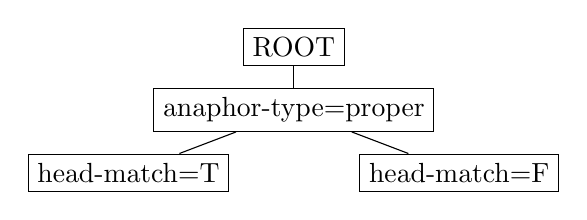
\begin{tikzpicture}
\node [rectangle,draw]{ROOT} [level distance=8mm,sibling distance=25mm]
child { node [rectangle,draw]{anaphor-type=proper} [level distance=8mm ,sibling distance=42mm]
child {node [rectangle,draw] {head-match=T}  [level distance=8mm ,sibling distance=27mm]
}
child {node [rectangle,draw] {head-match=F}}
};
\end{tikzpicture}
}
\end{center}
\caption[The final FP-Tree with support values]{A sample FP-Tree.\label{fp-tree_example}}
\end{figure}
\fi
\subsection{Informativeness Measures}
\label{patternEval}
%Similar to other supervised pattern mining approaches, 
%our goal is to select a set of patterns that is discriminative regarding the class label.
%Selected patterns also should not include redundant information. 
We use a \emph{discriminative power} and an \emph{information novelty} measure for determining informativeness.
We also use a \emph{frequency} measure which determines the required minimum frequency of a pattern in training samples.
It helps to avoid overfitting to the properties of the training data.

%We use the statistical significance of the association of a pattern and the class label 
%as the measure for choosing discriminative patterns. 
%We use the binomial test for choosing patterns with novel information.
%The binomial test is successfully used in previous work for mining discriminative patterns \cite{batal10}. 
%TODO
%The \emph{discriminative power} and \emph{information novelty} measures are partly checked during mining and also in the {post-processing} step. 
%This decreases the number of patterns for the post-processing step considerably, and therefore the time efficiency of the whole algorithm increases.
%The evaluation of the measures in the post-processing step
%is done in a more strict way.
%
 \noindent\textbf{Discriminative power}: We use the $G^2$ likelihood ratio test \cite{agresti07} in order to 
choose patterns whose association with the class variable 
is statistically significant.\footnote{A pattern is considered discriminative if 
the corresponding p-value is less than a fixed threshold ($0.01$).}
The $G^2$ test is successfully used for text analysis \cite{dunning93}.
%$G^2$ can be unreliable for expected frequencies of less than five \cite{agresti07}.
%However, since we experiment on large datasets and evaluate the significance measure 
%on patterns satisfying the frequency condition (Equation~\ref{eq:freq} or \ref{eq:freq_2}), 
%this problem does not apply in our case.
%If one is interested in rare patterns of data, Fisher's exact test is a better choice.
%However, Fisher's exact test is very slow in comparison to the $G^2$ test for large values of $n_{ij}$.
%


 \noindent \textbf{Information Novelty}:
%Hence, we should also ensure that 
%the selected relevant patterns provide novel information.
A large number of redundant patterns 
can be generated by adding irrelevant items to a base pattern that is discriminative itself.
%This leads to a large set of patterns
%conveying similar information.
%Many of these patterns may also be significant by themselves.
We consider the pattern $p$ as novel if (1) $p$ predicts the target class label $c$ significantly
better than all of its containing items, and 
(2) $p$ predicts $c$ significantly better than all of its sub-patterns that 
satisfy the frequency, discriminative power,  
and the first information novelty conditions.
Similar to \newcite{batal10}, we employ 
%a one-sided significance test using 
a binomial distribution to determine information novelty.
%
\subsection{Mining Algorithm}
\label{mining}
%
%Now we have all the ingredients needed to mine useful patterns of data as classification features.
The EPM algorithm is summarized in Algorithm~\ref{mine_patt}.
It takes FP-Tree $T$, pattern $p$ on which $T$ is conditioned, 
and set of items ($A_j \subset A$) whose combinations with $p$ will be examined. 
Initially, $p$ is empty and the FP-Tree is constructed based on all frequent items of data
and $A_j = A$. Resulting patterns are collected in $P$.

For each $a_i \in A_j$, the algorithm builds new pattern $q$ by combining $a_i$ with $p$.
$frequent(q)$ checks whether $q$ meets the frequency condition.
If $q$ is frequent, the algorithm continues the search process.
Otherwise, it is not possible to build any frequent pattern out of a non-frequent one.
\emph{Discriminative power} and the first condition of \emph{information novelty} are then checked for pattern $q$.
\begin{algorithm}[htp]
\SetAlgoLined
\DontPrintSemicolon 
\SetAlFnt{\small}
%\KwIn{$T$: input $\mathop{FP\mhyphen Tree}$}
%\KwIn{$p$: pattern base on which $T$ is conditioned}
%\KwIn{$A_j$: set of items to be combined with $p$}
%\KwOut{$P$: set of output patterns}
\SetKwFunction{algo}{$EPM$}
\SetKwProg{myalg}{Algorithm}{}{}
  \myalg{\algo{$T$, $p$, $A_j$}}{
  \ForEach {$a_i \in A_j$}{
  $q = p \cup \{a_i$\} \;
  \If{$Frequent(q)$}{
      \If{$Discriminative(q)$}{
	  %$testCount(|q|)+=1$ \;
	  \If{$Novel(q)$}{
	      $P = P \cup q$ \;
	  }
      }
      
      \If{$|q| >= \Theta_l$}{
	continue\;
      }
      \text{construct $T_{q}$ = $q$'s conditional tree} \;
      \vspace*{-.4cm}
       $EPM(T_{q}, q, ancestors(a_i))$ \;
   }
   }
   %\Return \text{Post-Prune(P)} \;
   \vspace*{0.1cm}
}
\caption{The EPM algorithm.}
\label{mine_patt}
\end{algorithm}

We use a threshold ($\Theta_l$) 
for the maximum length of mined patterns.
$\Theta_l$ can be set to large values if more complex and specific patterns are desirable.
%This threshold considerably reduces the search space, 
%especially for datasets with many features.

If $|q|$ is smaller than $\Theta_l$,
the conditional FP-Tree $T_{q}$ is built that represents patterns of $T$ that include the pattern $q$.
The mining algorithm then continues 
to recursively search for more specific patterns by combining $q$ with the items included in $ancestors(a_i)$,
which keeps the list of all ancestors of $a_i$ in the original FP-Tree.
%$ancestors$ is built while constructing the original FP-Tree.
EPM examines all frequent patterns of up to length $\Theta_l$. 
%

%\subsection{Post-Processing}
%The post-processing step checks \emph{discriminative power} and \emph{information novelty} in a more strict way.
%As mentioned in Section~\ref{mininFeatureg}, p-value is set to 0.01 ($\Theta_{p_0}$) during the pattern mining step. 
If we use a statistical test multiple times, the risk of making false discoveries increases \cite{webb2006}.
To tackle this, we apply the Bonferroni correction for multiple tests in a post-pruning function after the mining process.
%Similar to \newcite{bay2001}, we set the p-value threshold for all patterns of length $l$ as follows:
%\begin{equation}
%\Theta_{p_l} = min(\frac{\Theta_{p_0}}{2^l \times testCount(l)}, \Theta_{p_{l-1}}), \nonumber
%\end{equation}
%where $testCount(l)$ is the number of times that the $G^2$ test is applied on a pattern of length $l$.
This function also applies the second information novelty condition on the resulting patterns.
%Using the information novelty criteria in our pattern selection technique
%results into a less redundant set of patterns.